In this section, the basic GeoPAT procedures are presented. These are: 

\begin{itemize}
	\item {\bf Search} - search for areas similar to a query
	\item {\bf Change detection} - comparison of local patterns between two maps
	\item {\bf Segmentation} - division of a map into regions of cohesive patterns
	\item {\bf Clustering} - grouping patterns that are similar to each other
\end{itemize}

The procedures are explained using the workflow schemes and examples.
The examples how to process categorical data are shown on a $42\times 69$ km ($1400\times 2300$ px) part of the National Land Cover Dataset (NLCD) covering area around the city of Augusta, GA (Figure \ref{FIG:AUGUSTA}).
This area is characterized by high diversity of land cover categories and patterns.
Thus it is perfect for various pattern analyzes.

\begin{figure}[H]
	\centering
	\includegraphics[width=\textwidth]{atlanta.png}
	\caption{Part of NLCD, covering area around Augusta, GA used in the examples}
	\label{FIG:AUGUSTA}
\end{figure}

Examples of time-series analysis are based on monthly sums of precipitation for area of Great Britain from the WorldClim database (Figure \ref{FIG:PRCP}).
It consists of twelve raster files, where each file has 240 rows and 319 columns.
Precipitation values are expressed in milimeters.

\begin{figure}[H]
	\centering
	\includegraphics[width=\textwidth]{prcp.png}
	\caption{Monthly sums of precipitation for area of Great Britain used in the time-series examples}
	\label{FIG:PRCP}
\end{figure}

\FloatBarrier

\subsection{Search}

Search functionality enables user to produce maps of similarity. 
These maps show the level of similarity between a specified motifel (query) and a grid of motifels.
The input is one or more GeoTIFF raster maps (depending on a data and signature type; see appendix \ref{signatures} for more information), and XY coordinates of one or more points in space.
The result is one or more GeoTIFF raster maps which have the same extent as the grid of motifels specified by user.
The number of resulting maps is the same as the number of points provided.
The workflows for categorical and time series maps differ.

\subsubsection{Search on categorical maps}
Figure \ref{FIG:SEARCH} presents general workflow path for producing similarity maps using a categorical raster data. 

\begin{figure}[H]
	\centering
	\includegraphics[width=\textwidth]{search_scheme.png}
	\caption{Workflow path for search on categorical maps}
	\label{FIG:SEARCH}
\end{figure}

The first step is to prepare signature files for both, grid of motifels and query motifels, using two separate modules, {\it gpat\_gridhis} and {\it gpat\_pointshis} respectively. 
The second step is to use these signature files as inputs to {\it gpat\_search} module in order to the produce similarity maps.\\\\

{\bf Example:}

\begin{minipage}{\linewidth}
\begin{lstlisting}
gpat_gridhis -i Augusta2011.tif -o grid -s cooc -z 50 -f 50 -n pdf
gpat_pointshis -i Augusta2011.tif -o query_signatures.txt -s cooc -z 50 -n pdf --xy_file=coordinates.txt
gpat_search -i grid -r query_signatures.txt
\end{lstlisting}
\end{minipage}

For example, we can search for the most similar motifels to those located in the four points in the Figure \ref{FIG:SEARCH1}. 
Firstly, we need to build a grid of a motifels of a desired signature, size, shift, etc. 
Secondly, query motifels are extracted using a set of coordinates as an input. 
Finally, we can obtain the maps of similarity by comparing the grid from the first step with the query motifels from the second step.
The four final maps (Figure \ref{FIG:SEARCH2} shows similarity to each of the given points, where the brightest color indicates the most similar areas and the darkest color indicates the least similar areas.

\begin{figure}[H]
	\centering
	\includegraphics[width=\textwidth]{searchhis_plot1.png}
	\caption{Points of interest on the top of a landcover map}
	\label{FIG:SEARCH1}
\end{figure}

\begin{figure}[H]
	\centering
	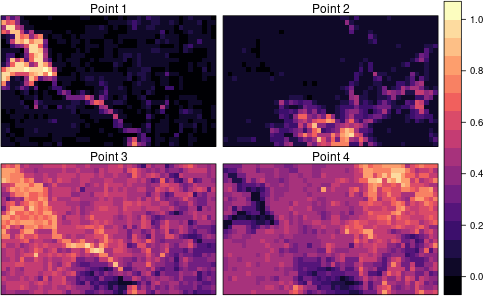
\includegraphics[width=\textwidth]{searchhis_plot2.png}
	\caption{Output similarity maps}
	\label{FIG:SEARCH2}
\end{figure}

\FloatBarrier

\subsubsection{Search on time series}
Figure \ref{FIG:SEARCHTS} presents general workflow path for producing similarity maps using a time-series raster data. 

\begin{figure}[H]
	\centering
	\includegraphics[width=\textwidth]{searchts_scheme.png}
	\caption{Workflow path for search on time series.}
	\label{FIG:SEARCHTS}
\end{figure}

The first step is to prepare signature files for both, grid of motifels and query motifels, using two separate modules, {\it gpat\_gridts} and {\it gpat\_pointsts} respectively. 
The second step is to use these signature files as inputs to {\it gpat\_search} module in order to the produce similarity maps.\\\\

{\bf Example:}

\begin{minipage}{\linewidth}
\begin{lstlisting}
gpat_gridts -i GB_pr01.tif -i GB_pr02.tif -i GB_pr03.tif -i GB_pr04.tif -i GB_pr05.tif -i GB_pr06.tif -i GB_pr07.tif -i GB_pr08.tif -i GB_pr09.tif -i GB_pr10.tif -i GB_pr11.tif -i GB_pr12.tif -o GB_pr_grid -n
gpat_pointsts -i GB_pr_grid -o query_signatures_ts.txt --xy_file=coordinates_gb.txt
gpat_search -i GB_pr_grid -r query_signatures_ts.txt -m tsEUC
\end{lstlisting}
\end{minipage}

For example, we want to find out which cities in Great Britain have the most (and the least) similar temporal pattern of precipitation. 
For this purpose, we need to have maps of precipitation (e.g. twelve rasters with montly sums of precipitation from January to December) and coordinates of our points of interest (Figure \ref{FIG:SEARCHTS1}).

\newpage

\begin{wrapfigure}{l}{0.35\textwidth}
	\includegraphics[width=0.33\textwidth]{searchts_plot1.png}
	\caption{Location of the points of interest}
	\label{FIG:SEARCHTS1}
\end{wrapfigure}

Firstly, a grid which contains temporal patterns of precipitation need to be built based on the precipitation rasters.

Secondly, query signatures are extracted based on the coordinates of points of interest - in our case cities of London, Glasgow, Cardiff, Fort William, and Dublin. 

Finally, we can create the maps of similarity (one for each city). 
To do so, we need to specify the similarity measure proper for time series data, such as {\it tsEUC} (time series - euclidean distance).
Our final five maps show where the annual precipitation patterns are the most and the least similar to those in our selected cities (Figure \ref{FIG:SEARCHTS2}). \\\\\\\\\\

\begin{figure}[H]
        \begin{center}
	\includegraphics[width=0.75\textwidth]{searchts_plot2.png}
	\caption{Maps of the similarity in terms of precipitation time-series}
	\label{FIG:SEARCHTS2}
        \end{center}
\end{figure}

\FloatBarrier

\subsection{Change detection}

Change detection module provides a way to compare patterns between two grids-of-scenes.
The output map show the level of similarity between two inputs.
Figure \ref{FIG:CHANGE} presents general workflow path for producing maps of change. 

\begin{figure}[H]
	\centering
	\includegraphics[width=\textwidth]{compare_scheme.png}
	\caption{Workflow path for change detection.}
	\label{FIG:CHANGE}
\end{figure}

The first step is to prepare signature files for both dataset, using either {\it gpat\_gridhis} for categorical data or {\it gpat\_gridts} for time series data.
The second step is to use these signature files as inputs to the {\it gpat\_compare} module in order to the produce change maps. \\\\

{\bf Example:}

\begin{minipage}{\linewidth}
\begin{lstlisting}
gpat_gridhis -i Augusta2006.tif -o Augusta2006_grid100 -z 100 -f 100
gpat_gridhis -i Augusta2011.tif -o Augusta2011_grid100 -z 100 -f 100
gpat_compare -i Augusta2006_grid100 -i Augusta2011_grid100 -o Augusta0611_compared.tif
\end{lstlisting}
\end{minipage}

For example, we want to compare a change in land cover patterns between years 2006 and 2011. 
For this purpose, we can use a landcover data from NLCD for 2006 and 2011 (Figure \ref{FIG:CHANGEDET1}).
Both of these datafiles need to have the same extent and resolution.

Firstly, we need to create a grid of signatures for both GeoTIFF files.
It is important to remember that both of the created grid of signatures must by created using the same size, shift, and signature.

\begin{figure}[H]
	\centering
	\includegraphics[width=\textwidth]{change_det_two_maps.png}
	\caption{Land cover maps of Augusta for year 2006 and 2011}
	\label{FIG:CHANGEDET1}
\end{figure}

Secondly, the output map is created based on the grids of signatures.
The final map shows where a land cover pattern stayed the same (value of 1) and where it changed. 
The lowest values indicate the biggest change of a land cover pattern.

\begin{figure}[H]
	\centering
	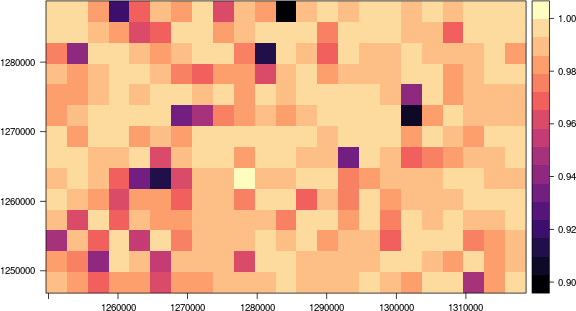
\includegraphics[width=\textwidth]{change_det.png}
	\caption{Maps of the similarity between a land cover of Augusta between 2006 and 2011}
	\label{FIG:CHANGEDET2}
\end{figure}

\FloatBarrier

\subsection{Segmentation}

Segmentation module enables user to create maps of segments.
Each of the output segment is internally homogeneous in terms of encapsulated pattern and, at the same time, different from the adjecent segments.
The input is a grid of signatures.
The result is a raster (GeoTIFF) and vector (ESRI Shapefile) file containing the segments.
Quality of segmentation could be also determined with raster maps of inhomogeneity, isolation, and overall quality.
Figure \ref{FIG:SEGMENT} presents general workflow path for segmentation. 

\begin{figure}[H]
	\centering
	\includegraphics[width=\textwidth]{segment_scheme.png}
	\caption{Workflow path for segmentation.}
	\label{FIG:SEGMENT}
\end{figure}

\subsubsection{Segmentation on categorical maps}



{\bf Example:}

\begin{minipage}{\linewidth}
\begin{lstlisting}
gpat_gridhis -i Augusta2011.tif -o Augusta2011_grid100 -z 100 -f 100
gpat_segment -i Augusta2011_grid100 -o Augusta2011_seg100.tif -v Augusta2011_seg100.shp  --lthreshold=0.1 --uthreshold=0.3
gpat_segquality -i Augusta2011_grid100 -s Augusta2011_seg100.tif -g Augusta2011_seg100_ih.tif -o Augusta2011_seg100_is.tif
\end{lstlisting}
\end{minipage}

\begin{figure}[H]
	\centering
	\includegraphics[width=\textwidth]{augusta2011_seg.png}
	\caption{Segments of landcover patterns of 3km scale for Augusta}
	\label{FIG:SEG1}
\end{figure}

\begin{figure}[H]
	\centering
	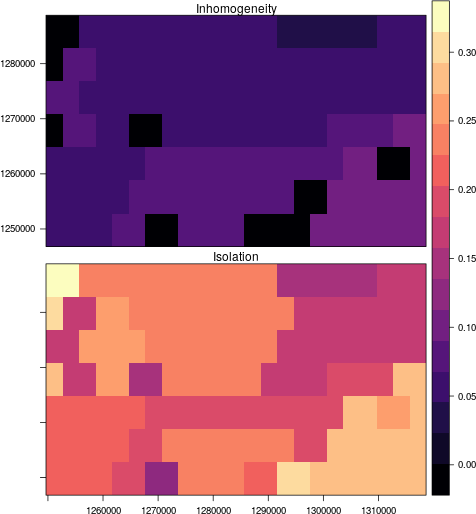
\includegraphics[width=\textwidth]{segmentation_quality.png}
	\caption{Inhomogenety and isolation metrics for the segmentation output}
	\label{FIG:SEG2}
\end{figure}

\begin{figure}[H]
	\centering
	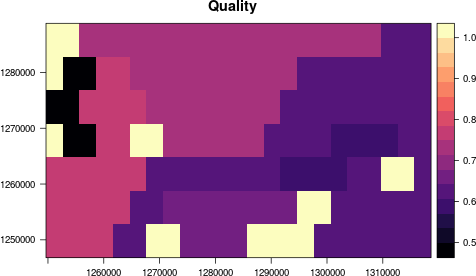
\includegraphics[width=\textwidth]{segmentation_qualityall.png}
	\caption{Quality of the segmentation of landcover patterns}
	\label{FIG:SEG3}
\end{figure}

% segmentation quality value (??) 0.7077751
% more likely 0.8229831

\FloatBarrier

\subsubsection{Segmentation on time series}

{\bf Example:}

\begin{minipage}{\linewidth}
\begin{lstlisting}
gpat_gridts -i GB_pr01.tif -i GB_pr02.tif -i GB_pr03.tif -i GB_pr04.tif -i GB_pr05.tif -i GB_pr06.tif -i GB_pr07.tif -i GB_pr08.tif -i GB_pr09.tif -i GB_pr10.tif -i GB_pr11.tif -i GB_pr12.tif -o GB_pr_grid -n
gpat_segment -i GB_pr_grid -o GB_pr_seg.tif -v GB_pr_seg.shp -m tsEUC --lthreshold=0.5 --uthreshold=1
gpat_segquality -i GB_pr_grid -s GB_pr_seg.tif -g GB_pr_seg_ih.tif -o GB_pr_seg_is.tif -m tsEUC
\end{lstlisting}
\end{minipage}

% create a side panel

\begin{wrapfigure}{r}{0.5\textwidth}
	\centering
	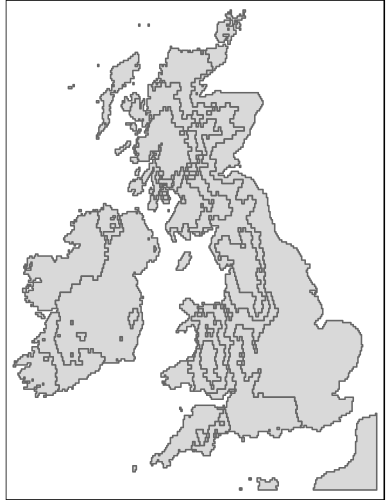
\includegraphics[width=0.4\textwidth]{ts_seg.png}
	\caption{Segments of the montly precipitation temporal patterns for Great Britain}
	\label{FIG:SEGTS1}
\end{wrapfigure}

\begin{wrapfigure}{r}{0.5\textwidth}
\end{wrapfigure}

\begin{figure}[H]
	\centering
	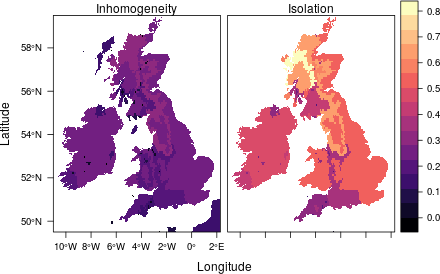
\includegraphics[width=\textwidth]{ts_segmentation_ihis.png}
	\caption{Inhomogenety and isolation metrics for the segmentation of the montly precipitation temporal patterns for Great Britain}
	\label{FIG:SEGTS2}
\end{figure}

\begin{figure}[H]
	\centering
	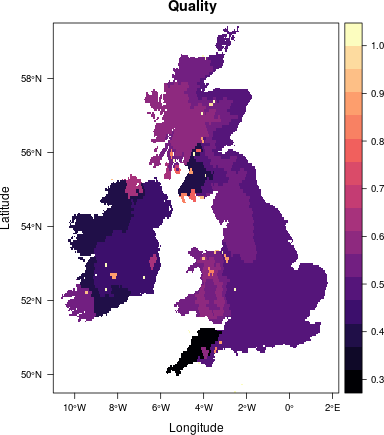
\includegraphics[width=\textwidth]{ts_segmentation_qualityall.png}
	\caption{Quality of the segmentation of the montly precipitation temporal patterns for Great Britain}
	\label{FIG:SEGTS3}
\end{figure}

% segmentation quality value (??) 0.5353301
% more likely 0.6709943

\FloatBarrier

\subsection{Clustering}
Work in progress...

\subsubsection{Clustering of individual motifels}

\begin{figure}[H]
	\centering
	\includegraphics[width=\textwidth]{cluster_points_scheme.png}
	\caption{Workflow path for clustering of motifels.}
	\label{FIG:CLUSTER_POINTS}
\end{figure}

\begin{figure}[H]
	\centering
	\includegraphics[width=\textwidth]{cluster_pointsts_scheme.png}
	\caption{Workflow path for clustering of time series motifels.}
	\label{FIG:CLUSTER_POINTSTS}
\end{figure}

\FloatBarrier

\subsubsection{Clustering of grid of motifels}

\begin{figure}[H]
	\centering
	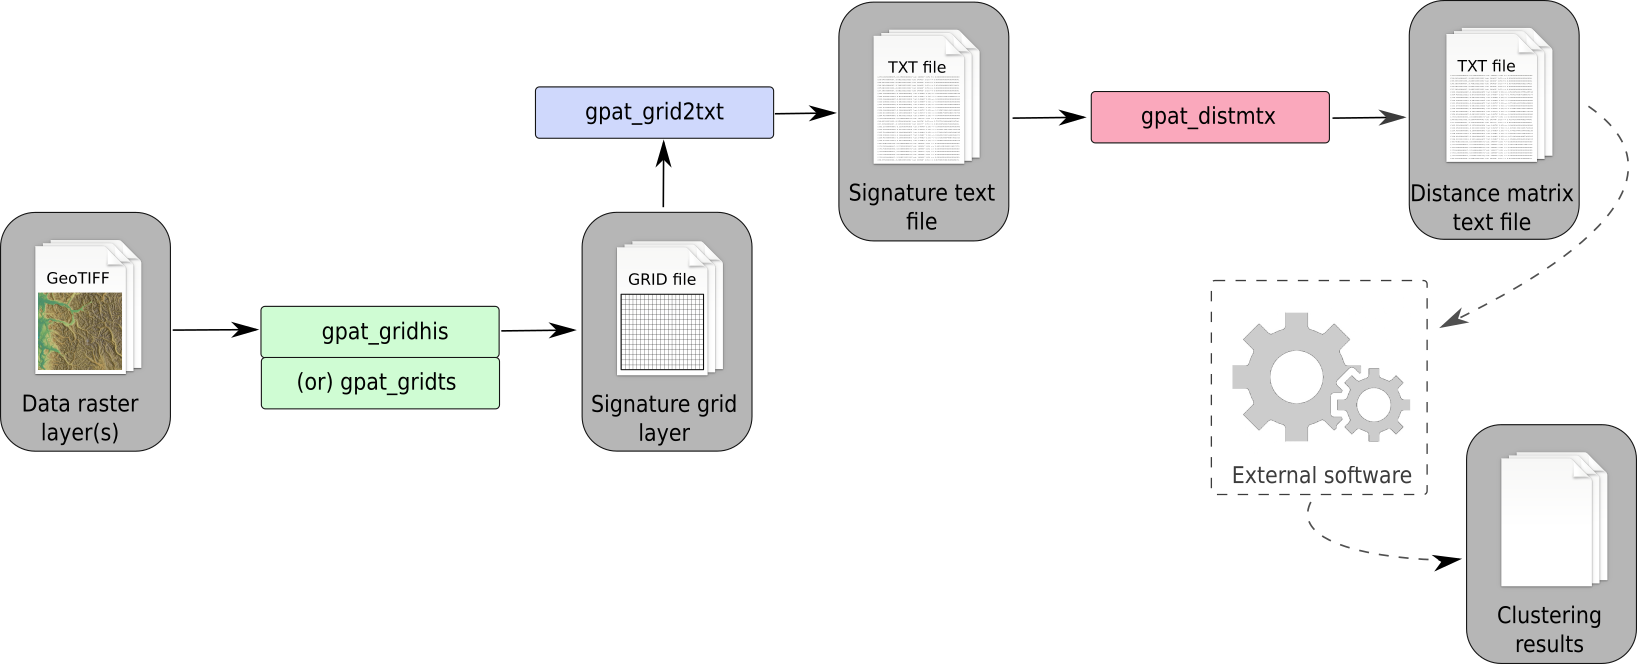
\includegraphics[width=\textwidth]{cluster_grid_scheme.png}
	\caption{Workflow path for clustering of grid of motifels.}
	\label{FIG:CLUSTER_GRID}
\end{figure}

\FloatBarrier

\subsubsection{Clustering of segments / predefined irregular regions}

\begin{figure}[H]
	\centering
	\includegraphics[width=\textwidth]{cluster_seg_scheme.png}
	\caption{Workflow path for clustering of segments (regions).}
	\label{FIG:CLUSTER_SEGMENT}
\end{figure}